
\subfloat[16-APSK]{
%% 16-APSK Modulation Constellation
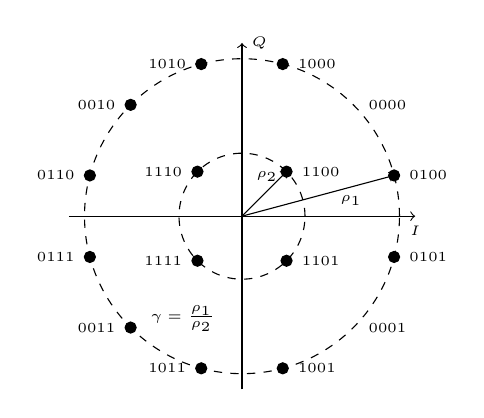
\begin{tikzpicture}[scale=1]

    \tikzstyle{every node}=[font=\tiny]
    \def\cos45{0.7071}
    \def\rad{.8cm}
    \def\RAD{2cm}
    \colorlet{anglecolor}{black}

    \draw[dashed] (0,0) circle (\rad);
    \draw[dashed] (0,0) circle (\RAD);
    \draw[->] (-2.2,0) -- (2.2,0) node[below] {$I$};
    \draw[->] (0,-2.2) -- (0,2.2) node[right] {$Q$};

    \filldraw [black] (45:\rad) circle(2pt)
                     (-45:\rad) circle(2pt)
                     (135:\rad)  circle(2pt)
                     (-135:\rad)  circle(2pt)
                     (135:\RAD)      circle(2pt)
                     (225:\RAD)      circle(2pt)
                     (15:\RAD)       circle(2pt)
                     (-15:\RAD)       circle(2pt)
                     (-75:\RAD)       circle(2pt)
                     (75:\RAD)       circle(2pt)
                     (105:\RAD)       circle(2pt)
                     (165:\RAD)       circle(2pt)
                     (-165:\RAD)       circle(2pt)
                     (-105:\RAD)       circle(2pt)
                     (-165:\RAD)       circle(2pt);

     \draw[->] (0,0)--(15:\RAD);
     \draw[->] (0,0) -- (45:\rad);
     \draw (45:\rad) node[right=2pt] {$1100$};
     \draw (-45:\rad) node[right=2pt] {$1101$};
     \draw (135:\rad) node[left=2pt] {$1110$};
     \draw (225:\rad) node[left=2pt] {$1111$};
     \draw (45:\RAD) node[right=2pt] {$0000$};
     \draw (15:\RAD) node[right=2pt] {$0100$};
     \draw (75:\RAD) node[right=2pt] {$1000$};
     \draw (-15:\RAD) node[right=2pt] {$0101$};
     \draw (-45:\RAD) node[right=2pt] {$0001$};
     \draw (-75:\RAD) node[right=2pt] {$1001$};
     \draw (105:\RAD) node[left=2pt] {$1010$};
      \draw (135:\RAD) node[left=2pt] {$0010$};
      \draw (165:\RAD) node[left=2pt] {$0110$};
      \draw (-165:\RAD) node[left=2pt] {$0111$};
      \draw (-135:\RAD) node[left=2pt] {$0011$};
      \draw (-105:\RAD) node[left=2pt] {$1011$};
      \draw (8:1.4) node {$\rho_1$};
      \draw (58:.6) node {$\rho_2$};
      \draw (-120:1.5) node {$\gamma = \frac{\rho_1}{\rho_2}$};
\end{tikzpicture}
}\qquad
\subfloat[32-APSK]{
%% 32-APSK Modulation Constellation
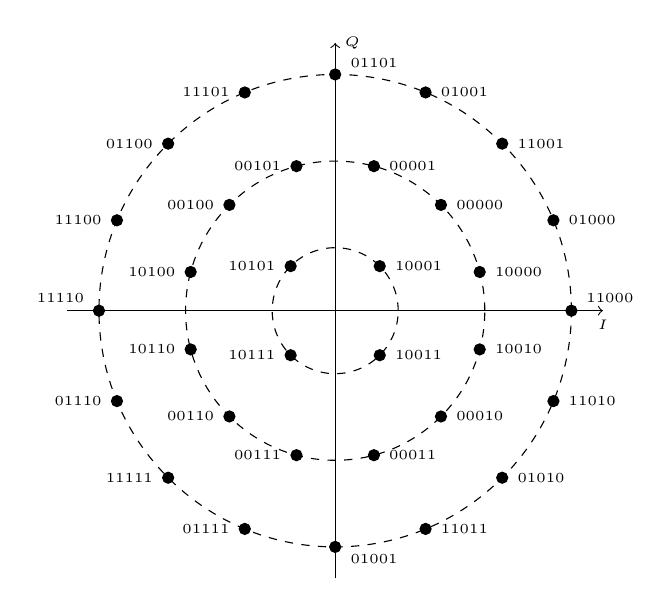
\begin{tikzpicture}[scale=1]

    \tikzstyle{every node}=[font=\tiny]
    \def\cos45{0.7071}
    \def\rad{.8cm}
    \def\RAD{3cm}
    \def\RaD{1.9}
    \colorlet{anglecolor}{black}

    \draw[dashed] (0,0) circle (\rad);
    \draw[dashed] (0,0) circle (\RaD);
    \draw[dashed] (0,0) circle (\RAD);
    \draw[->] (-3.4,0) -- (3.4,0) node[below] {$I$};
    \draw[->] (0,-3.4) -- (0,3.4) node[right] {$Q$};

    \filldraw [black] (45:\rad) circle(2pt)
                     (-45:\rad)  circle(2pt)
                     (-135:\rad)   circle(2pt)
                     (135:\rad)   circle(2pt)
                     (15:\RaD)      circle(2pt)
                      (45:\RaD)      circle(2pt)
                     (75:\RaD)      circle(2pt)
                     (105:\RaD)      circle(2pt)
                     (135:\RaD)      circle(2pt)
                     (165:\RaD)       circle(2pt)
                     (-15:\RaD)      circle(2pt)
                      (-45:\RaD)      circle(2pt)
                     (-75:\RaD)      circle(2pt)
                     (-105:\RaD)      circle(2pt)
                     (-135:\RaD)      circle(2pt)
                     (-165:\RaD)       circle(2pt)
                     (0:\RAD)          circle(2pt)
                     (22.5:\RAD)       circle(2pt)
                     (45:\RAD)       circle(2pt)
                     (67.5:\RAD)       circle(2pt)
                     (90:\RAD)       circle(2pt)
                     (112.5:\RAD)       circle(2pt)
                     (135:\RAD)       circle(2pt)
                     (157.5:\RAD)       circle(2pt)
                     (180:\RAD)       circle(2pt)
                     (-22.5:\RAD)       circle(2pt)
                     (-45:\RAD)       circle(2pt)
                     (-67.5:\RAD)       circle(2pt)
                     (-90:\RAD)       circle(2pt)
                     (-112.5:\RAD)       circle(2pt)
                     (-135:\RAD)       circle(2pt)
                     (-157.5:\RAD)       circle(2pt);
                     

     %\draw[->] (0,0)--(15:2.6cm);
%     \draw[->] (0,0) -- (\cos45, \cos45);
     \draw (45:\rad)  node[right=2pt] {$10001$};
     \draw (-45:\rad) node[right=2pt] {$10011$};
     \draw (135:\rad) node[left=2pt] {$10101$};
     \draw (225:\rad) node[left=2pt] {$10111$};
     \draw (15:\RaD) node[right=2pt] {$10000$};
     \draw (45:\RaD) node[right=2pt] {$00000$};
     \draw (75:\RaD) node[right=2pt] {$00001$};
     \draw (105:\RaD) node[left=2pt] {$00101$};
     \draw (135:\RaD) node[left=2pt] {$00100$};
     \draw (165:\RaD) node[left=2pt] {$10100$};
     \draw (-15:\RaD) node[right=2pt] {$10010$};
     \draw (-45:\RaD) node[right=2pt] {$00010$};
     \draw (-75:\RaD) node[right=2pt] {$00011$};
     \draw (-105:\RaD) node[left=2pt] {$00111$};
     \draw (-135:\RaD) node[left=2pt] {$00110$};
     \draw (-165:\RaD) node[left=2pt] {$10110$};
     
     
     \draw (22.5:\RAD) node[right=2pt] {$01000$};
     \draw (45:\RAD) node[right=2pt] {$11001$};
     \draw (67.5:\RAD) node[right=2pt] {$01001$};
     \draw (90:3.15cm) node[right=2pt] {$01101$};
      \draw (112.5:\RAD) node[left=2pt] {$11101$};
      \draw (135:\RAD) node[left=2pt] {$01100$};
      \draw (157.5:\RAD) node[left=2pt] {$11100$};
      \draw (177:\RAD) node[left=2pt] {$11110$};
      \draw (3:\RAD) node[right=2pt] {$11000$};
      \draw (-22.5:\RAD) node[right=2pt] {$11010$};
     \draw (-45:\RAD) node[right=2pt] {$01010$};
     \draw (-67.5:\RAD) node[right=2pt] {$11011$};
     \draw (-90:3.15cm) node[right=2pt] {$01001$};
      \draw (-112.5:\RAD) node[left=2pt] {$01111$};
      \draw (-135:\RAD) node[left=2pt] {$11111$};
      \draw (-157.5:\RAD) node[left=2pt] {$01110$};
      %\draw (12:2.2) node {$\rho_1$};
%      \draw (38:.8) node {$\rho_2$};
%      \draw (-120:1.8cm) node {$\gamma = \frac{\rho_1}{\rho_2}$};
\end{tikzpicture}
}